\documentclass[a4paper, 10pt]{report}

% metadata
% ---------------------------------------------------------------------------

\newcommand{\name}{Naoki Pross}
\newcommand{\instructor}{Rinaldo Geiler, Daniele Kamm}
\newcommand{\specialization}{S.2 Sviluppare prototipi}

\newcommand{\project}{Spectrum Analyzer}
\newcommand{\projstart}{12.04.2018}
\newcommand{\projend}{15.05.2018}
\newcommand{\projectyear}{2017-18}

\newcommand{\plannedtime}{83 UD}
\newcommand{\actualtime}{-- UD}

% ---------------------------------------------------------------------------
% layout
\usepackage[
    inner=3cm,
    outer=3cm,
    top=3.5cm,
    bottom=3.5cm
]{geometry}

\usepackage{fancyhdr}
\pagestyle{fancy}
\fancyhf{}
\fancyhead[L]{CAM-SAM}
\fancyhead[C]{Elettronico}
\fancyhead[R]{\today}
\fancyfoot[L]{\jobname.tex}
\fancyfoot[C]{\name}
\fancyfoot[R]{\thepage}

\usepackage{afterpage}
\usepackage{titlesec}

\titleformat{\chapter}[hang]{\Huge\bfseries}
    {\thechapter}{.5em}{\thispagestyle{fancy}}
\titlespacing*{\chapter}{0pt}{-30pt}{10pt}

% language
\usepackage[italian]{babel}

% quotes
\usepackage{csquotes}
\usepackage{fancyvrb}

% sans serif font
\renewcommand{\familydefault}{\sfdefault}

% urls
\usepackage[
    colorlinks=true,
    linkcolor=.,
    urlcolor=blue
]{hyperref}

% maths
\usepackage{amsmath}
\usepackage{amssymb}
\usepackage{amsthm}

% figures
\usepackage{float}
\usepackage{subfig}
% tables
\usepackage{array}
\usepackage{booktabs}
\usepackage{tabularx}
% plots
\usepackage{pgfplots}
% diagrams
\usepackage{tikz}
\usepackage[european]{circuitikz}
\usepackage{tikz-timing}
\usepackage{tikzscale}

% code
\usepackage{xcolor}
\usepackage{listings}
\lstdefinestyle{cc}{
    belowcaptionskip=1\baselineskip,
    breaklines=true,
    frame=none,
    % margin
    xleftmargin=\parindent,
    % numbers
    numbers=left,
    numbersep=5pt,
    numberstyle=\ttfamily\footnotesize\color{gray},
    %
    language=C,
    showstringspaces=false,
    % font
    basicstyle=\ttfamily\normalsize,
    keywordstyle=\color{green!40!black},
    commentstyle=\color{gray},
    identifierstyle=\color{black},
    stringstyle=\color{orange},
}
\lstset{escapechar=`, style=cc}

% ---------------------------------------------------------------------------
\numberwithin{equation}{subsection}
\newcommand{\dd}[1]{\mathrm{d}#1}

% ---------------------------------------------------------------------------
\begin{document}

    \begin{titlepage}
\thispagestyle{empty}
\newgeometry{margin=3cm}
\renewcommand{\arraystretch}{1.5}

\begin{tikzpicture}[remember picture,overlay]
    \node[anchor=north west, inner sep=0pt] 
        at ($(current page.north west)+(3cm, -3cm)$) {
            
\includegraphics[height=2.25cm]{figures/logo/LOGO_SAM}
        };
\end{tikzpicture}

\begin{flushright}
    \LARGE \bfseries
    Anno scolastico \projectyear \\
    Lavoro Professionale Individuale
\end{flushright}

\large
\begin{tabularx}{\textwidth}{l X}
    \midrule
    Nome Cognome: & \textbf{\name} \\

    \midrule
    Professione: & \textbf{Elettronico} \\

    \midrule
    Titolo del progetto: & \textbf{\project} \\

    \midrule
\end{tabularx}
\vfill

% immagine opizonale
% \includegraphics[\height=]{figures}

\vfill
\begin{tabularx}{\textwidth}{l X l X}
    \midrule
    Azienda: & \multicolumn{3}{l}{\parbox{5cm}{
        \textbf{CPT Bellinzona} \\
        Centro d'arti e mestieri \\
        Viale S. Franscini 25 \\
        6500 Bellinzona%
    }} \\

    \midrule
    Formazione approfondita: & \multicolumn{3}{l}{\textbf{\specialization}} \\

    \midrule
    Formatore: & \multicolumn{3}{l}{\textbf{\instructor}} \\

    \midrule
    Data d'inizio: & \textbf{\projstart} & Ore a disposizione: & \textbf{\plannedtime}\\

    \midrule
    Data file lavoro: & \textbf{\projend} & Ore effettive: &  \textbf{\actualtime} \\

    % \midrule
    % Data di compilazione & \textbf{\today} \\

    \midrule
\end{tabularx}

\restoregeometry
\end{titlepage}

    \tableofcontents

	% spacing between paragraphs
	\setlength{\parskip}{.5em}

	\chapter{Introduzione}

\section{Contesto}
Per portare a termine il percorso formativo per un attestato di capacit\`a
federale presso la Scuola Arti e Mestieri di Bellinzona \`e richiesto lo
sviluppo individuale di un progetto di produzione di un prodotto.
Per interesse personale nella matematica della trasformata di Fourier mi \`e
stato assegnato di sviluppare un analizzatore spettrale.

\section{Requisiti}
\`E richiesto di sviluppare circuito per analizzare lo spettro dei segnali di
frequenza fino a 10\,kHz. Il dispositivo dovr\`a avere 3 possibili sorgenti:
RCA/Cinch e 2 Audio Jack per un microfono e per una sorgente di audio
generica. \`E inoltre richiesto che il calcolo dei dati dello spettrogramma
sia eseguito da un microcontroller della Microchip, collegato a due
altri dispositivi quali, un display e ad un computer in RS232, per poter
visualizzare lo spettrogramma computato.

\section{Concetti matematici}
Il circuito realizzato si appoggia sul concetto matematico di importanza
fondamentale, nelle discipline come la fisica e l'elettrotecnica della
\emph{Trasformata di Fourier}. Questa operazione matematica \`e fondata su
un principio dimostrato da Joseph Fourier che asserisce che \`e possibile
rappresentare una qualsiasi funzione periodica, in alcuni casi anche non
periodica, con una serie di sinusoidi di frequenze multiple ad una di base.
L'operazione di \emph{Trasformata} dunque \`e uno strumento per osservare
le frequenze di queste armoniche, esso trasforma una funzione in funzione del
tempo \(f(t)\) in una funzione rispetto alla frequenza o alla pulsazione
\(\hat f(\omega)\), che restituisce ad ogni \(\omega\) l'ampiezza e la fase
dell'armonica.

Secondariamente, il progetto usufruisce anche di un altro strumento chiamato
\emph{Fast Fourier Transform} (FFT) scoperto inizialmente nel 1965 dai
matematici J. Cooley e J. Tukey. La FFT \`e un algoritmo con molte
implementazioni che riduce la complessit\`a computazionale della trasformata
di fourier discreta da \(\mathcal{O}(n^2)\) a \(\mathcal{O}(n \log n)\).
Questo \`e necessario perch\'e le operazioni matematiche da eseguire sono dei
prodotti tra numeri complessi, i quali impiegano molto tempo per essere
computati.

Tutti i concetti descritti saranno approfonditi nei capitoli seguenti.

\section{Norme di progetto}
%\subsection{Software}
{\renewcommand\arraystretch{1.2}
\begin{table}[H] \centering
    \caption{Norme di progetto: Software}
    \begin{tabularx}{\textwidth}{X l}
        \toprule
        \bfseries Componente & \bfseries Software \\
        \midrule
        Version control  & Git \\
        Documentazione   & \textrm{\LaTeX} \\
        Diario di lavoro & \textrm{\LaTeX} \\
        Pianificazione   & MS Excel 2016 \\
        \midrule
        \textrm{\LaTeX} engine & \textrm{\XeLaTeX} \\
        ECAD                   & Altium Designer 2017 \\
        Embedded toolchain     & Microchip XC, MPLabX \\
        Desktop Toolchain      & QtCreator, g++, MinGW \\
        \bottomrule
    \end{tabularx}
\end{table}
}

%\subsection{Hardware}
Per i valori non specificati sono utilizzati i predefiniti del software ECAD.
{\renewcommand\arraystretch{1.2}
\begin{table}[H] \centering
    \caption{Norme di progetto: Hardware}
    \begin{tabularx}{\textwidth}{X r l}
        \toprule
        \bfseries Regola & \bfseries Valore & \bfseries Unit\`a \\
        \midrule
        Number of Layers        &   2 & -- \\
        Silkscreen / Overlay    &  No & -- \\ 
        Minimum trace width     &  30 & mil \\
        Maximum trace width     &  60 & mil \\
        Minimum trace clearance &  20 & mil \\
        Minimum power rail width & 50 & mil \\
        Minimum pad diameter    &  80 & mil \\
        Minimum pad hole diameter & 25 & mil \\
        \bottomrule
    \end{tabularx}
\end{table}
}

%\subsection{Programmazione}
\begin{table}[H] \centering
    \caption{Norme di progetto: Programmazione}
    \begin{tabularx}{\textwidth}{X l}
        \toprule
        \bfseries Regole per programmazione embedded & \\
        \midrule
        Paradigma & Imperativo sequenziale \\
        Convenzione per i nomi & \texttt{snake\_case}, sempre minuscolo \\
        Tabulatore & 4 spazi \\
        Tabulato con gli spazi & S\`i \\
        \midrule
        \bfseries Regole per programmazione desktop & \\
        \midrule
        Paradigma  & Imperativo ad oggetti (OOP) \\
        Convenzione per i nomi & Convenzioni di Qt \\
        Tabulatore & 4 spazi \\
        Tabulato con gli spazi & S\`i \\
        \bottomrule
    \end{tabularx}
\end{table}

	\chapter{Hardware}
\section{Schema a blocchi}

\begin{figure}[H] \centering \rmfamily
    \tikzstyle{block} = [draw, thick, fill=gray!10, rectangle, minimum height=3em, minimum width=6em]
    \begin{tikzpicture}[auto, node distance=3cm,>=latex']

        \coordinate (mic) at (0,1);
        \coordinate (jack) at (0,0);
        \coordinate (cinc) at (0,-1);

        \node[block, right of=jack, minimum height=9em] (mux) {MUX};
        \node[block, right of=mux] (ampl) {Amplifier};
        \node[block, right of=ampl] (filter) {LP Filter};
        \node[block, right of=filter, node distance=4cm] (mcu) {MCU};

        \node[block, below of=mcu, node distance=2cm] (dpy) {Display};
        \node[block, above of=mcu, node distance=2cm] (pc) {Computer};

        \draw[->] (mic) -- node {Mic} (mux.west |- mic);
        \draw[->] (jack) -- node {Jack} (mux.west |- jack);
        \draw[->] (cinc) -- node {Cinc} (mux.west |- cinc);

        \draw[->] (mux.east) -- node {\(u\)} (ampl.west);
        \draw[->] (ampl.east) -- (filter.west);
        \draw[->] (filter.east) -- node {\(H(j\omega)\,u\)}(mcu.west);

        \draw[->] (mux.north) ++(0,1) node [above] {S} -- (mux.north);
        \draw[->] (ampl.north) ++(0,1) node [above] {G} -- (ampl.north);

        \draw[->] (mcu.south) -- (dpy.north);
        \draw[->] (mcu.north) -- node {\small RS232}(pc.south);
    \end{tikzpicture}
    \caption{Schema a blocchi}
\end{figure}

\section{Selezione delle entrate}
Essendo richiesta dai requisiti la possibilit\`a di selezione tra 3 entrate,
\`e stato utilizzando un semplice multiplexer controllato direttamente dal
microcontroller. Per la sua semplicit\`a non sono necessari particolari
osservarzioni.

\begin{figure}[H] \centering
    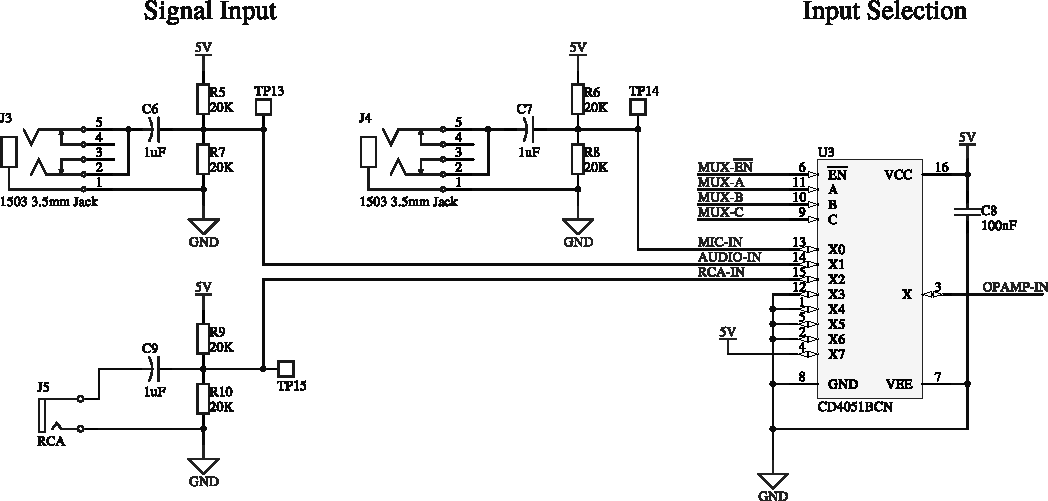
\includegraphics[width=.8\linewidth]{figures/circuits/input-selection.pdf}
    \caption{Circuito di selezione delle entrate \label{fig:input-selection}}
\end{figure}

Tutte le entrate dispongono di un condensatore di disaccoppiamento seguito da
un partitore di tensione simmetrico per aggiungere un offset pari a met\`a
dell'alimentazione. Il valore delle resistenze di 20\,k\(\Omega\) \`e scelto
per avere un impedenza rispetto al connettore uguale all'impedenza
caratteristica dei cavi audio di 10\,k\(\Omega\).

\section{Circuito di entrata}
Il segnale di cui si analizza lo spettro, prima di essere campionato, viene
adattato mediate un circuito di amplificazione e filtraggio. Esso \`e
necessario per due ragioni. Il circuito di amplificazione \`e presente per
poter regolare il circuito nel caso in cui si dovesse avere in entrata un
segnale di ampiezza molto piccola. Il secondo circuito invece, di filtraggio,
\`e necessario per rimuovere disturbi di alta frequenza che potrebbero
introdurre disturbi nel campionamento. Questa \`e una tipica configurazione
prima di un circuito di conversione AD (analogico - digitale), ed \`e
conosciuto anche come circuito di filtraggio \emph{anti-alias}.

\begin{figure}[H] \centering
    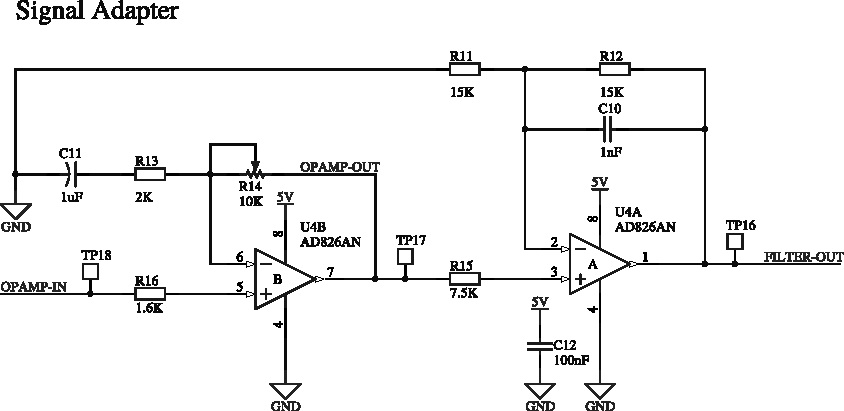
\includegraphics[width=.8\linewidth]{figures/circuits/filter-ampl.pdf}
    \caption[Circuito di adattamento del segnale]{
        Circuito di adattamento del segnale in entrata.
        \label{fig:filter-ampl}
    }
\end{figure}

\`E importante notare che per questa applicazione si \`e scelto utilizzare
degli opamp \emph{rail to rail}\footnote{Vedi sezione \ref{sec:err-opamp}},
che hanno una tensione di saturazione vicina a quella di alimentazione. Essi
sono necessari per poter raggiungere tensioni vicino allo 0\,V, che non
sarebbero possibili con un opamp normale siccome l'alimentazione del circuito
\`e asimmetrica tra 0 e 12\,V.

\paragraph{Amplificatore.} Come si pu\`o notare a sinistra nella figura
\ref{fig:filter-ampl}, il circuito di amplificazione non ha una configurazione
tipica. Esso \`e basato su una configurazione non invertente ma dispone di un
consensatore (C11) che modifica la retroazione in modo da reagire unicamente
alla componente AC del segnale. Questo permette di amplificare la componente
alternata ignorando l'offset del segnale, perci\`o di \emph{non} utilizzare
un'alimentazione simmetrica \(\pm\)5\,V.

L'amplificazione di questo amplificatore \`e comunque data dal rapporto
\(1+R_{14}/R_{13}\) che permette un un guadagno fino a 6 oppure 15,5\,dB.


\paragraph{Filtro.} A destra della figura \ref{fig:filter-ampl} vi \`e il
circuito di filtraggio, realizzato utilizzando un tipico filtro passa basso
attivo di primo ordine. Esso \`e dimensionato con una frequenza di taglio di
10\,kHz poich\`e quest'ultimo \`e il limite di Nyquist, conosciuto anche dal
teorema di Shannon, il quale stata che la frequenza di campionamento deve
essere almeno doppia della frequenza dell'armonica di frequenza maggiore.

Anche il filtro essendo non invertente ha un rapporto di amplificazione dato
da \(1+R_{12}/R_{11}\). Nella figura il valore della resistenza \(R_{11}\) \`e
\textbf{incorretto} (Vedi sezione \ref{sec:err-filter}). Dopo la correzzione
(\(R_{11} \geq 750\,\textrm{k}\Omega\)) il filtro ha un amplificazione
approssimativamente unitaria (\(\approx 1.02\)).

\section{Microcontroller}
Per questa applicazione \`e stato deciso di utilizzare il microcontroller a 8
bit di Microchip PIC18F45K22, principalmente per la sua frequenza di lavoro.
Questo PIC senza oscillatori esterni dispone di un clock a 16\,MHz che grazie
ad un PLL interno pu\`o essere aumentata fino a ad un massimo di 64\,MHz.

Inoltre questo microcontroller dispone di un moltiplicatore hardware 8x8 che
impiega un solo ciclo, risparmiando la difficolt\`a di dover ottimizzare le
computazioni della Fast Fourier Tranform.

Un ultima ragione importante per la scelta di questo componente \`e data dalla
disponibilit\`a di una libreria per controllare il la matrice LED, utilizzata
per la visualizzazione, adattata da Arduino da P. Randjelovic in un LPI
precedente.

In allegato \`e presente una pagina riassuntiva dal datasheet.

 \section{Visualizzazione}

	\chapter{Software}
\section{Campionamento} \label{sec:sampling}
Per campionare il segnale \`e stato scelto di utilizzare il TIMER2, sia per la
sua semplicit\`a che per la granulati\`a offerta dal registro di comparazione.
Il campionamento \`e eseguito ad una frequenza di 20\,kHz, poco sotto al
valore massimo possibile che si pu\`o ottenere considerando il tempo di
conversione dell'ADC.

\begin{figure}[H] \centering
    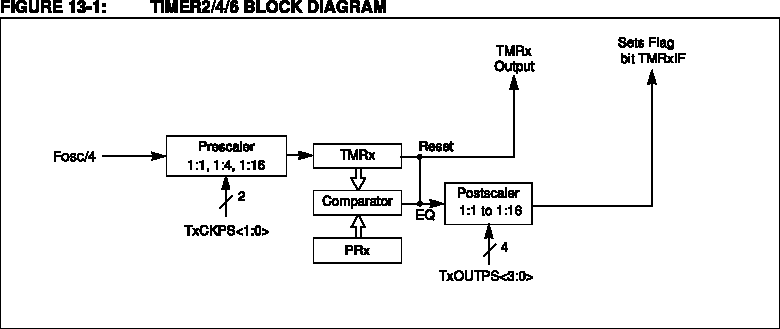
\includegraphics[width=.9\linewidth]{figures/timer2-block-diagram}
    \caption[Schema a blocchi del TIMER2]{
        Schema a blocchi del TIMER2. Fonte: Microchip PIC18F2X/4XK22 datasheet
        \label{fig:timer2-diagram}
    }
\end{figure}

Dallo schema a blocchi nella figura \ref{fig:timer2-diagram}, si pu\`o
osservare che la frequenza degli interrupt, ossia di campionamento, \`e data
dalla seguente relazione.
\[
    f = \frac{F_{osc}}{4}\cdot
        \frac{1}{\textrm{prescaler}}\cdot
        \frac{1}{\textrm{comparator}}\cdot
        \frac{1}{\textrm{postscaler}}
\]
Per il questo progetto il PIC18F45K22 \`e configurato con un postscaler 1:1 ed
un prescaler 1:16, per far corrispondere un unit\`a del comparatore ad 1
microsecondo. Perci\`o il comparatore \`e impostato a 50, poich\`e
\(1/50\,\mu\textrm{s} = 20\,\textrm{kHz}\).
\[ 
    f = \frac{64\,\textrm{MHz}}{4}\cdot
        \frac{1}{1}\cdot
        \frac{1}{\textrm{comparator}}\cdot
        \frac{1}{16}
      = \frac{1\,\textrm{MHz}}{\textrm{comparator}} 
      = \frac{1\,\textrm{MHz}}{50} = 20\,\textrm{kHz}
\]
In allegato la figura \ref{fig:embedded-flowchart} mostra il diagramma di
flusso del programma.

\section{Trasferimento dei dati}
Per trasferire i dati campionati era inizialmente stato scelto di utilizzare
una struttura dati binaria. In seguito per\`o si \`e deciso di utilizzare un
formato interamente ASCII per semplificare il debugging.

\begin{figure}[H] \centering
    \begin{tikzpicture}[
            timing/yunit=5mm,
            timing/xunit=4mm,
            timing/text format={\Large \ttfamily},
            timing/.style={black}
        ]
        \timing at (0,0) {
            LL
            3D{S\textbackslash n\textbackslash r}
            4D{\(a_0\)}
            1D{i}
            4D{\(b_0\)}
            2D{\textbackslash n\textbackslash r}
            4D{\(a_1\)}
            1D{i}
            4D{...}
            3D{E\textbackslash n\textbackslash r}
            LL
        };
    \end{tikzpicture}
    \caption[Protocollo di trasmissione dei dati]{
        Protocollo di trasmissione dei dati, il primo dato mandato \`e
        \(a_0+ib_0\)
        \label{fig:proto}
    }
\end{figure}
I dati sono trasferiti con un semplice protocollo illustrato nella figura
\ref{fig:proto}. Un frame di dati incomincia con il carattere ASCII maiuscolo
`S' seguito da un line break (\texttt{\textbackslash n\textbackslash r}). Ogni
riga seguente \`e un numero complesso a 4 cifre con il carattere `i' come
separatore tra la parte immaginaria e complessa (Es: \texttt{0140i0670\\n\\r}).
Il frame termina con il carattere ASCII maiuscolo `E' seguito da un line break.

La trasmissione di basso livello \`e gestita dalla porta EUSART del
microcontroller, impostato per funzionare in modalit\`a asincrona con i dati
da 8 bit, 1 stop bit ad una velocit\`a di 57600 bps.

\section{Interfaccia al Computer}
Per preferenze principalmente personali \`e stato scelto di realizzare
l'interfaccia al computer utilizzando il moderno linguaggio di programmazione
C++ (versione \(\geq\) 11) utilizzando un framework (Qt) che sar\`a descritto
successivamente.  I vantaggi dati dall'utilizzo del C++ anzich\`e linguaggi
interpretati come il Python, linguaggi compilati in bytecode come Java, o con
runtime particolari come LabView / CVI sono molteplici. Innanzitutto tutti gli
strumenti necessari per lo sviluppo hanno mezzi o varianti \emph{open source /
libre}, di conseguenza gratuiti e in molti casi multipiattaforma. Al contrario
invece dei sistemi proprietari come quelli offerti da National Instruments che
sono estremamente costosi e possono essere utilizzati unicamente sulle
piattaforme con un supporto ufficiale.  Tra i vari linguaggi di programmazione
non proprietari il C++ \`e comunque in posizione di vantaggio siccome \`e tra
i pi\`u performanti in quanto non richiede alcun interpreter (bytecode o non)
o nessuna runtime, stando quindi alla pari con il linguaggio C guadagnando
per\`o i vantaggi dell'astrazione data dalla programmazione ad oggetti.

\subsection{Librerie e codice di terzi}
Per ridurre i tempi dedicati alla realizzazione del programma, seppur
mantenendo una buona qualit\`a, \`e stato scelto di utilizzare le seguenti
librerie.

\begin{itemize}
    \item Serial (\url{http://wjwwood.io/serial/}): Utilizzata come
        interfaccia multipiattaforma per l'accesso di basso livello alla porta
        seriale del sistema operativo sottostatante. Descrizione dal sito:
        \begin{displayquote}
            This is a cross-platform library for interfacing with rs-232
            serial like ports written in C++. It provides a modern C++
            interface with a workflow designed to look and feel like PySerial,
            but with the speed and control provided by C++. 
        \end{displayquote}

    \item QCustomPlot (\url{http://qcustomplot.com}): Utilizzata per produrre
        il grafico all'interno del software, per visualizzare i dati dal
        microcontroller. Descrizione dal sito:
        \begin{displayquote}
            QCustomPlot is a Qt C++ widget for plotting and data
            visualization. It has no further dependencies and is well
            documented. This plotting library focuses on making good looking,
            publication quality 2D plots, graphs and charts, as well as
            offering high performance for realtime visualization applications. 
        \end{displayquote}
\end{itemize}

\subsection{Qt Framework}
La dipendenza principale utilizzata per realizzare la grafica \`e il framework
di Qt. Inoltre Qt \`e un'azienda indipendente che vende un supporto
commerciale per lo sviluppo di applicazioni su praticamente ogni piattaforma.
Qt \`e un framework grafico maturo che esiste oramai da 22 anni ed \`e
disponibile sia con una licenza commerciale che con le licenze open source
LGPL e GPL.

La toolchain di Qt aggiunge al normale sviluppo un preprocessore speciale
chiamato MOC che genera in automatico il codice dalle strutture grafiche
realizzate con QtDesigner. Il resto della toolchain \`e composta da componenti
tipici che possono essere intercambiati liberamente poich\`e Qt supporta
gcc/g++, clang, MSVC e MinGW. Per compilare il codice \`e dunque necessario un
compiler qualsiasi di C++ e l'IDE QtCreator, oppure qmake. Questi ultimi due
pacchetti offrono il preprocessore MOC. Per progetti open source entrambi sono
offerti gratuitamente dal sito ufficiale \url{www.qt.io}.

\subsection{Compilazione sotto Linux}
Il programma \`e stato realizzato in parte sotto Debian 9.4 Stretch ed in
parte sotto Fedora 27. Per entrambi i sistemi sono necessarie le dipendenze
per lo sviluppo di Qt5.

\noindent Una volta installate le dipendenze dalla cartella di progetto \`e
possibile utilizzare il makefile per compilare le dipendenze e il codice.
\begin{Verbatim}[frame=single]
$ make build-deps   # dependencies
$ make              # spectrum analyzer code 
\end{Verbatim}
Purtroppo la libreria QCustomPlot utilizza un sistema di build molto
particolare che richiede molte dipendenze. Perci\`o in alcuni casi \`e
preferibile scaricare dal seguente link l'ultima versione dei due files
\texttt{qcustomplot.cpp} e \texttt{qcustomplot.hpp} ed immetterli manualmente
nella cartella \texttt{lib/qcustomplot/}.
\begin{center}
\url{http://qcustomplot.com/index.php/download}
\end{center}
Ed infine si compila con
\begin{Verbatim}[frame=single]
$ make serial       # build only Serial library dep
$ make              # build spectrum analyzer code 
\end{Verbatim}

\subsection{Compilazione manuale sotto Linux}
Per compilare manualmente il progetto sono necessari pochi passaggi grazie a
qmake. Come per il caso precedente la libreria QCustomPlot pu\`o essere
scaricata dal sito.

\begin{enumerate}
\item Scaricare le dipendenze.
\begin{Verbatim}[frame=single]
$ git submodule init
$ git submodule update
\end{Verbatim}

\item Compilare la libreria Serial
\begin{Verbatim}[frame=single]
$ mkdir -p lib/build-serial
$ qmake -makefile -o Makefile -Wall "CONFIG+=releae" \
    -o lib/build-serial/ lib/serial

$ make -C lib/build-serial/
\end{Verbatim}

\item Compilare la libreria QCustomPlot
\begin{Verbatim}[frame=single]
$ cd lib/qcustomplot/src
$ sed -i -e 's/qmake474/qmake/' release.py
$ ./release.py
$ cd ../.. # go back to project root dir
\end{Verbatim}

\item Compilare il progetto
\begin{Verbatim}[frame=single]
$ mkdir -p build-deskop
$ qmake -makefile -o Makefile -Wall "CONFIG+=release" \
    -o build-desktop/ src-desktop

$ make -C build-desktop
\end{Verbatim}
\end{enumerate}

\subsection{Compilazione sotto Windows}
Per compilare il progetto in Windows \`e necessario installare QtCreator dal
sito ufficiale \url{www.qt.io}.

\begin{enumerate}
\item Installare QtCreator, Qt \(\geq\) 5.0 (consigliato 5.10.0)
\item Installare MinGW oppure MSVC + Visual Studio (consigliato MinGW)
\item Inizializzare ed aggiornare i submoduli di Git oppure clonare
    recursivamente il progetto.
\item Scaricare dal sito \url{http://qcustomplot.com/index.php/download} i
    documenti \texttt{qcustomplot.cpp} \texttt{qcustomplot.hpp} della libreria
    QCustomPlots ed immetterli nella cartella \texttt{lib/qcustomplots/}
\item Aprire il progetto \texttt{lib/serial/serial.pro} ed impostare la
    build directory sia per release che per debug in \texttt{lib/build-serial}.
\item Compilare la libreria Serial come release.
\item Aprire il progetto \texttt{src-desktop/SpectrumAnalyzer.pro} ed
    impostare la cartella di build sia per release che debug nella cartella
        \texttt{build-desktop/}
\item Compilare il progetto SpectrumAnalyzer come release
\item Controllare che lo script \texttt{deploy-desktop.cmd} abbia le variabili
    \texttt{QT\_PATH} e \texttt{QT\_VERSION} che corrispondano con la vostra
    l'installazione.
\item Eseguire lo script \texttt{deploy-desktop.cmd}.
\end{enumerate}
Nella cartella \texttt{build-desktop} sar\`a pronto l'eseguibile con tutte le
librerie dinamiche (DLL) necessarie.

\subsection{Architettura}
Il programma desktop \`e programmato per reagire ad eventi asincroni dati dalla
porta seriale del sistema operativo e dalle interazioni dell'utente.
La gestione degli eventi grafici \`e affidata interamente a Qt, perci\`o sono
stati scritti solamente i metodi che vengono attivati in funzione degli eventi
dall'utente.

Per la porta seriale invece il compito della gestione \`e stato delegato ad
una classe \texttt{SerialWorker} che ha un rapporto di \emph{composizione} con
la classe \texttt{MainWindow} in quanto essa esiste unicamente quando esiste
\texttt{MainWindow}. Nella figura \ref{fig:desktop-sequence} \`e mostrato un
diagramma delle sequenze che mostra il flusso dei dati attraverso le
componenti del programma.

Per l'implementazione nella figura \ref{fig:desktop-classes} \`e possibile
osservare il diagramma UML delle classi. \`E importante notare che Qt 
introduce dei nuovi tipi di membri chiamati \emph{slots} e \emph{signals}.
Gli slots sono dei normali metodi che rispondo ai signals. I signals invece
sono delle funzioni prive di implementazione che possono essere \emph{emesse}.

Quando viene realizzato un modello ad oggetti in Qt \`e possibile collegare
degli slots a dei segnali per poter gestire delle azioni asincrone.  Nel
progetto dello SpectrumAnalyzer il segnale \texttt{receivedData} della classe
\texttt{SerialWorker} viene messo quando sono stati ricevuti dei dati validi
dalla seriale. Il segnale ha come argomento un vettore di numeri complessi
interi.

Nella classe \texttt{MainWindow} il segnale di \texttt{receivedData} \`e
associato allo slot \texttt{serialDataReceiver} con argomento uguale al
segnale, dunque un vettore di numeri complessi interi, che processa i dati e li
mostra nell'interfaccia utente.

\begin{figure}[H] \centering
    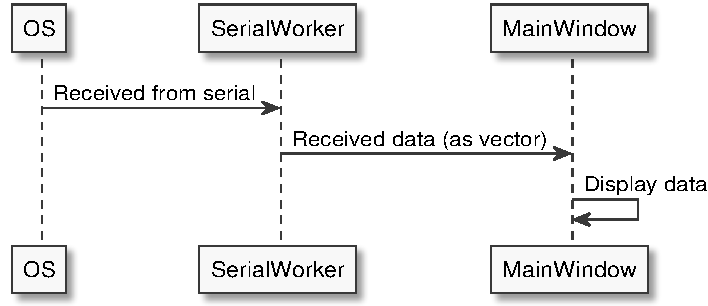
\includegraphics[width=.6\textwidth]{figures/uml/desktop-sequence}
    \caption{Diagramma delle sequenze \label{fig:desktop-sequence}}
\end{figure}

\begin{figure}[H] \centering
    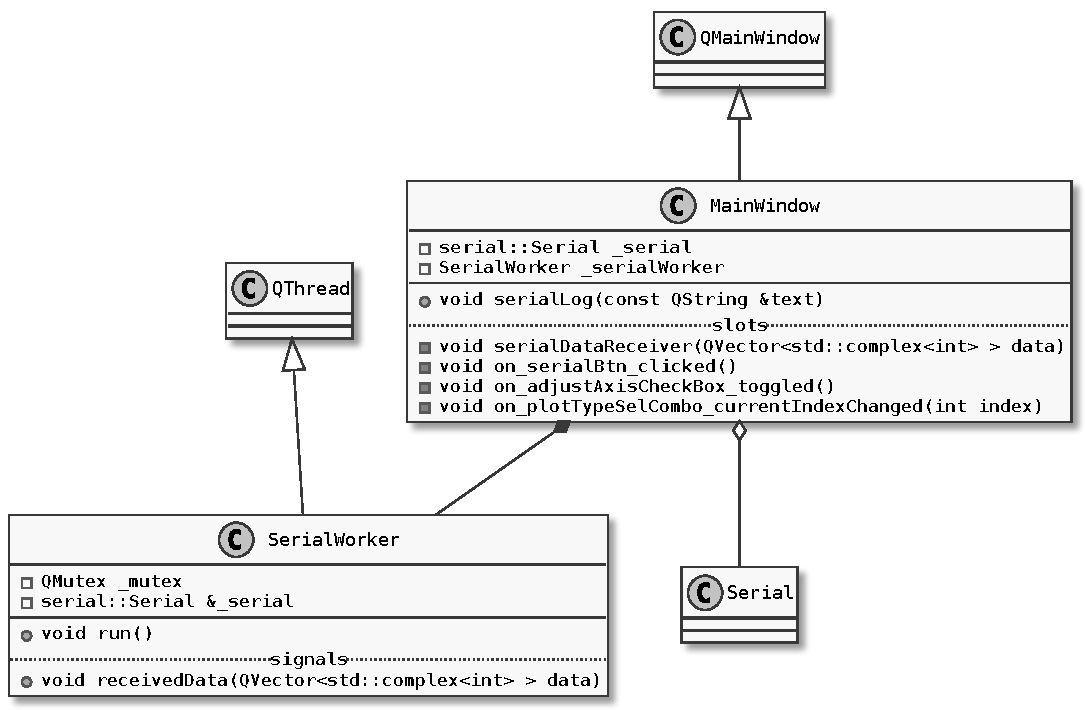
\includegraphics[width=\textwidth]{figures/uml/desktop-classes}
    \caption{Diagramma delle classi \label{fig:desktop-classes}}
\end{figure}

\subsection{Interfaccia utente}
L'interfaccia utente, realizzata con Qt \`e molto semplice e non dovrebbe
richiedere delle istruzioni d'utilizzo.
Dal software \`e possibile esportare i dati sia in formato CSV sia in un
immagine del grafico in formato vettoriale o bitmap / compresso (png, jpg).
\begin{figure}[H] \centering
	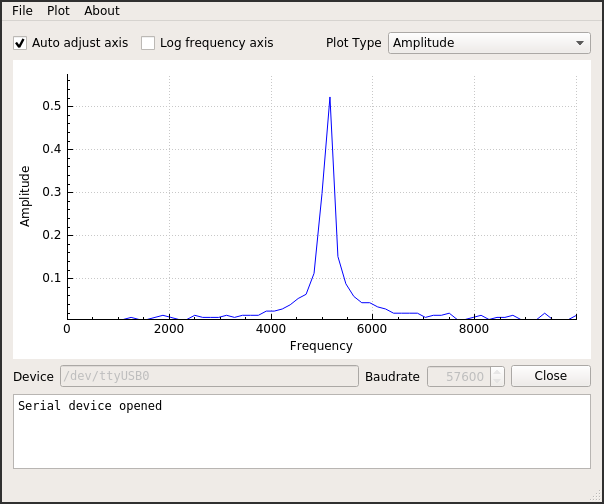
\includegraphics[width=.45\textwidth]{figures/screenshots/desktop-fedora-sine}
	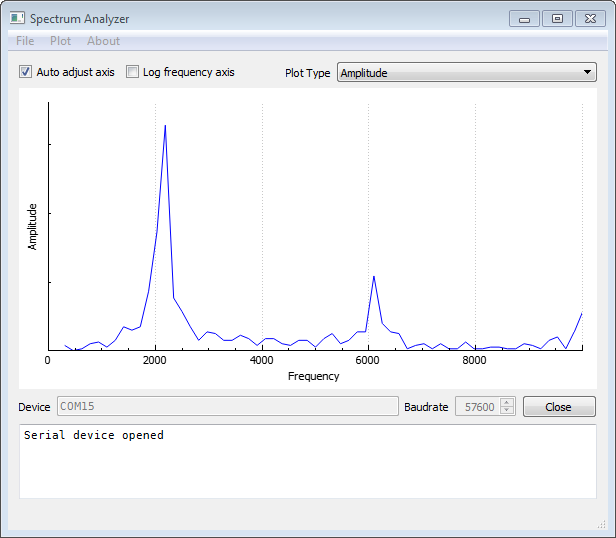
\includegraphics[width=.45\textwidth]{figures/screenshots/desktop-windows7-square}
    \caption{L'applicativo sotto Fedora 27 (sinistra) e Windows 7 (destra)}
\end{figure}
\begin{figure}[H] \centering
	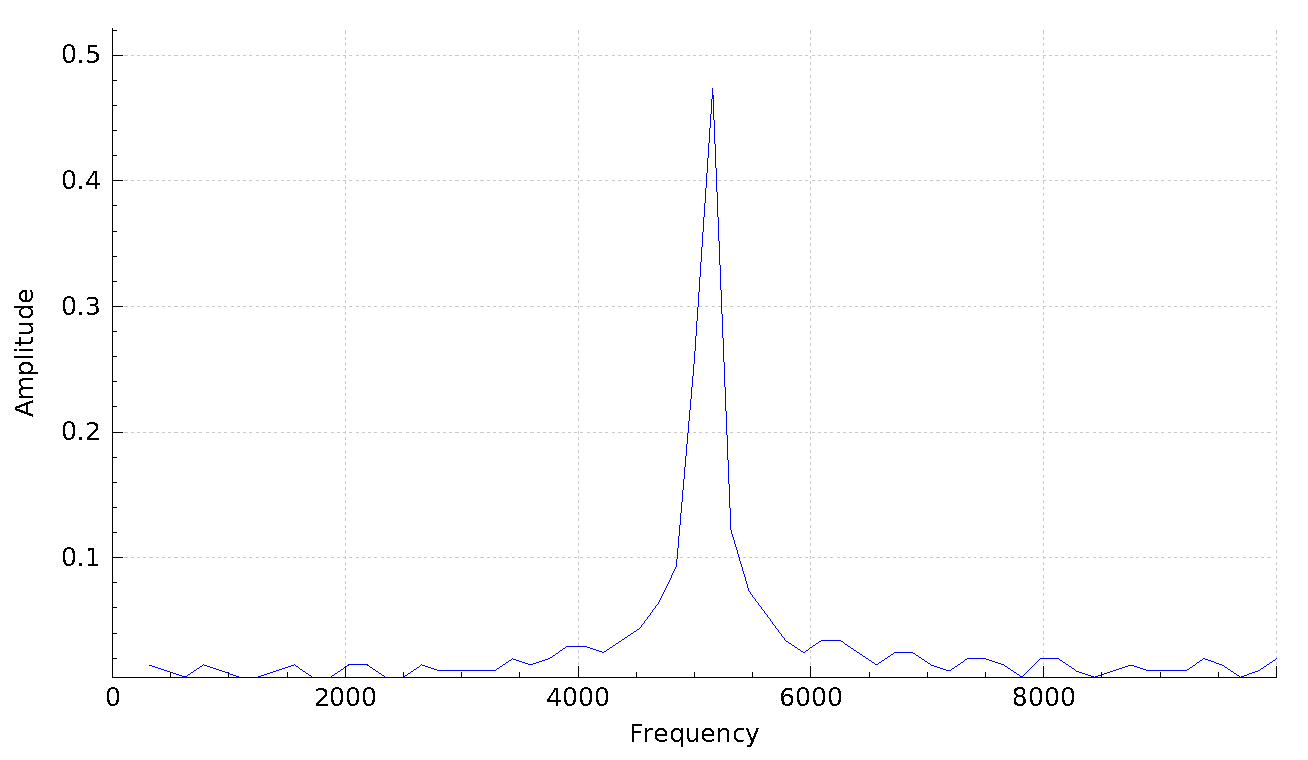
\includegraphics[width=.8\linewidth]{figures/screenshots/desktop-exported-sine-wave-img}
    \caption{Esempio di immagine esportata dal software}
\end{figure}

% \section{Interfaccia al Display}

\section{Fast Fourier Transform}
Il codice della FFT \`e stato preso dal dominio pubblico. Originalmente
scritto da Tom Roberts (8.11.1989), successivamente adattato da Malcom Stanley
(15.12.1994), Dimitrios P. Buras (14.6.2006) ed infine da Simon Inns
(4.1.2011) \cite{waitingforfriday} non ha praticamente necessitato modifiche.
L'algoritmo implementato \`e chiamato ``Fixed-Point in-place Fast Fourier''



	\chapter{Problemi riscontrati / Bugs}

    \begin{thebibliography}{2}
%\bibitem{example}
    % \textsc{Example item title},
    % (online), Author and other informations, \\
    % \url{https://www.example.com}

\bibitem{waitingforfriday}
    \textsc{Real Time Audio Spectrum Analyzer}. (online) 
    Simon Inns. Jan 8 2011. \\
    \url{https://www.waitingforfriday.com/?p=325} \\
    \url{http://archive.is/IJeAe} (archived)

\bibitem{mit-fft}
    \textsc{Divide and Couquer: FFT}. (online, video) \\
    Erik Demaine, MIT OpenCourseWare.
    MIT 6.046J Design and Analysis of Algorithms, Spring 2015 \\
    \url{https://youtu.be/iTMn0Kt18tg}

\bibitem{3blue1brown}
    \textsc{But what is the Fourier Transform? A visual introduction}. (online, video) \\
    Grant Sanderson. Jan 26, 2018. YouTube. \\
    \url{https://youtu.be/spUNpyF58BY}

\bibitem{signaux}
    \textsc{Théorie et traitement des signaux}. (Pag. 70 -- 72) \\
    Coulon, Frédéric de (1996).
    Lausanne: Presses polytechniques et universitaires romandes, 1996
    (Traité d'électricité de l'Ecole polytechnique fédérale de Lausanne; vol. 6)

\bibitem{minimiquadrati}
    \textsc{Algèbre linéaire. Aide-mémoire, exercices et applications}. (Pag.\,64 Moindres carrées) \\
    Dalang, Robert C. Chaabouni, Amel (2001). 
    Lausanne: Presses polytechniques et universitaires romandes, 2001

\bibitem{linearalgebra}
    \textsc{Algèbre linéaire}. (Pag 63 -- 65)\\
    Cairoli, R. (1991).
    Lausanne: Presses polytechniques et universitaires romandes, 1991

\bibitem{curtis}
    \textsc{Linear Algebra. An Introductory Approach.} \\
    Curtis, Charles W. (2000).
    New York: Springer, 2000


\bibitem{ftplot}
    \textsc{Example: Fourier transform}. (online)
    Jake. TeX.SE \\
    \url{http://www.pgfplots.net/tikz/examples/fourier-transform/}

\end{thebibliography}

\listoffigures
\begingroup
\let\clearpage\relax
\vspace{15mm}
\listoftables
\endgroup


	% allegati
    %\appendix
    \chapter{Trasformata di Fourier}

\section{Nozioni preliminarie}

\subsection{Regressione lineare con il metodo dei minimi quadrati}
La regressione lineare \`e un'approssimazione di una serie di dati ad una
funzione lineare. Questa retta di approssimazione pu\`o essere calcolata in
molteplici modi, per questo progetto \`e di interesse utilizzare il
\emph{metodo dei minimi quadrati}.  Sar\`a dunque esplicato come trovare i
coefficienti di una retta a \(m+1\) termini partendo da \(N\) punti di
riferimento.
\begin{equation}
    r(x, a_0, \dots, a_m) = a_0 + x\sum_{i=1}^{m}a_i
\end{equation}
Consideriamo di avere gli insiemi \(X\) e \(Y\) entrambi con \(N\) termini di
cui si prende le coppie ordinate di valori \((x_k, y_k)~ x_k\in X,\,y_k\in
Y\), ossia i punti dato di cui eseguire la regressione.  Il metodo dei minimi
quadrati trova i coefficienti della retta minimizzando il quadrato della
differenza tra il valore stimato dalla retta \(r(x_k)\) e il valore reale
\(y_k\).
\begin{equation*}
    \min((r(x_k) - y_k)^2)\quad \forall x_k\in X,\, y_k\in Y
\end{equation*}
Definiamo quindi la funzione da minimizzare \(\varepsilon\)
\begin{equation}
    \varepsilon(a_0, \dots, a_m) = \sum_{k=1}^{N}\Big[r(x_k, a_0, \dots, a_m)  - y_k\Big]^2
\end{equation}
Da cui si computa le derivati parziali rispetto ai coefficienti ricercati,
ottenendo un sistema di equazioni lineare. Ci\`o corrisponde anche ad
affermare che il \emph{gradiente} di \(\varepsilon\) \`e un vettore
\(\in\mathbb{R}^{m+1}\) con tutte le componenti a 0.
\begin{equation*}
    \nabla\varepsilon = \langle 0, \dots, 0 \rangle
\end{equation*}
A questo punto si pu\`o procedere risolvendo il sistema con l'algebra lineare
definendo la matrice di trasformazione \(\mathbf{A}\) e il vettore dei termini
noti \(\vec{u}\)
\begin{equation*}
    \nabla \varepsilon = \mathbf{A}
        \langle a_0, \dots,  a_m \rangle + \vec{u} \iff
    \langle a_0, \dots, a_m \rangle =
        \mathbf{A}^{-1}(-\vec{u})
\end{equation*}

\subsection{Funzione armonica}
Una funzione armonica, sinusoidale, pu\`o essere descritta in molteplici modi.
Iniziamo dunque osservando le forme pi\`u semplici, ossia la forma
trigonometrica.
\begin{align} \label{eq:harmonics-trig}
    f(x) &= a\cdot\sin (\omega x + \varphi) \\
    f(x) &= b\cdot\cos(\omega x + \vartheta)
\end{align}
Conoscendo la formula di Eulero \eqref{eq:euler}
\begin{equation} \label{eq:euler}
    e^{i\varphi} = \cos(\varphi) + i\cdot\sin(\varphi)
\end{equation}
possiamo riscrivere \(f(x)\) nei seguenti modi
\begin{align} \label{eq:harmonics-complex}
    f(x) &= \frac{a}{2i}\cdot(e^{i(x\omega + \varphi)} - e^{-i(x\omega + \varphi)}) \\
    f(x) &= \frac{b}{2}\cdot(e^{i(x\omega + \vartheta)} + e^{-i(x\omega + \vartheta)})
\end{align}

\subsection{Propriet\`a di ortogonalit\`a del seno e del coseno}
Per avere delle fondamenta solide prima dell'introduzione dell'argomento
principale, sar\`a dimostrata l'ortogonalit\`a delle due funzioni
trigonometriche mediante alcune verit\`a matematiche su degli integrali
definiti.  Per tutti i casi seguenti definiamo \(T\) come il periodo della
funzione periodica.

\begin{align*}
    & \int_0^T \sin(\frac{m2\pi x}{T})\,\dd{x} = 0
        \quad \forall m \in \mathbb{Z} \\
    %
    & \int_0^T \cos(\frac{m2\pi x}{T})\,\dd{x} = 0
        \quad \forall m \in \mathbb{Z^*} \\
    %
    & \int_0^T \sin(\frac{m2\pi x}{T})\cos(\frac{n2\pi x}{T})\,\dd{x} = 0
        \quad \forall m,n \in \mathbb{Z} \\
    %
    & \int_0^T \sin(\frac{m2\pi x}{T})\sin(\frac{n2\pi x}{T})\,\dd{x} = 0 
        \quad \forall m,n \in \mathbb{Z}~|~m\neq \pm n \\
    %
    & \int_0^T \sin^2(\frac{m2\pi x}{T})\,\dd{x} = \frac{T}{2}
        \quad \forall m \in \mathbb{Z} \\
    %
    & \int_0^T \cos(\frac{m2\pi x}{T})\cos(\frac{n2\pi x}{T})\,\dd{x} = 0 
        \quad \forall m,n \in \mathbb{Z}~|~m\neq \pm n \\
    %
    & \int_0^T \cos^2(\frac{m2\pi x}{T})\,\dd{x} = \frac{T}{2}
        \quad \forall m \in \mathbb{Z^*} \\
\end{align*}

\subsubsection{Dimostrazioni}


\section{Polinomio Trigonometrico}


\section{Serie di Fourier}
La serie di Fourier, nominata tale in onore a Jean-Baptise Joseph Fourier, di
una funzione \`e descritta nel modo seguente.
\begin{equation} \label{eq:fourier-series}
    f(x) = a_0 + \sum_{n=1}^{\infty}\Big [
        a_n\cdot\cos(\frac{n2\pi x}{T}) +
        b_n\cdot\sin(\frac{n2\pi x}{T}) \Big ]
\end{equation}
Con questa equazione Fourier ha teorizzato che \`e possibile rappresentare
qualsiasi funzione come una combinazione lineare di armoniche di frequenze
multiple di una frequenza di base. Con la seguente identi\`a trigonometrica
\`e possibile anche descrivere la serie con una notazione pi\`u compatta.
\begin{equation*}
    a\cdot\cos(\alpha) + b\cdot\sin(\alpha) = A\cdot\cos(\alpha-\vartheta)
\end{equation*}
Per \(A = \sqrt{a^2+b^2}\), \(\cos(\vartheta)=\frac{b}{A}\) e
\(\sin(\vartheta)=\frac{b}{A}\). Dunque
\begin{align}
    f(x) &= a_0 + \sum_{n=1}^{\infty} 
        A_n\cdot\cos(\frac{n2\pi x}{T} - \vartheta_n) \\
    f(x) &= a_0 + \sum_{n=1}^{\infty} 
        A_n\cdot\sin(\frac{n2\pi x}{T} + \varphi_n)
\end{align}

\section{Trasformata di Fourier discreta}

\section{Trasformata di Fourier}

\section{Fast Fourier Transform}
\subsection{Motivazioni e Complessit\`a temporale}
\subsection{Propriet\`a dei numeri complessi}




\end{document}
